\documentclass[a4paper]{article}

%------------------------------------------------------------
\usepackage[a4paper, total={6in, 9in}]{geometry}
\usepackage{amsmath, amssymb}
\usepackage{booktabs}
\usepackage{caption}
\usepackage{enumitem}
\usepackage{graphicx}
\usepackage{float}
\usepackage{inconsolata}
\usepackage{listings}
\usepackage{mathtools}
\usepackage{pstricks-add}
\usepackage{siunitx}
\usepackage[most]{tcolorbox}
\usepackage{tikz, pgfplots}
\usepackage{epstopdf} %converting to PDF
\usepackage{hyperref}
\usepackage{xfrac}

\usetikzlibrary{shapes.geometric}
\usetikzlibrary{arrows}

%------------------------------------------------------------
\graphicspath{{./fig/}}
\pgfplotsset{compat=1.13}
%------------------------------------------------------------
\setlength{\parindent}{0in}

\lstdefinestyle{C++}{
	language=C++,
	basicstyle=\ttfamily,
	keywordstyle=\color{blue}\ttfamily,
	stringstyle=\color{red}\ttfamily,
	commentstyle=\color{green}\ttfamily,
	morecomment=[l][\color{magenta}]{\#},
	showstringspaces=false
}

%------------------------------------------------------------
\newtcblisting[auto counter]{sexylisting}[2][]{sharp corners, 
    fonttitle=\bfseries, colframe=gray, listing only, 
    listing options={basicstyle=\ttfamily,language=C++}, 
    title=Listing \thetcbcounter: #2, #1}

%------------------------------------------------------------
\lstset{language=C++,
        basicstyle=\ttfamily,
        keywordstyle=\color{blue}\ttfamily,
        stringstyle=\color{red}\ttfamily,
        commentstyle=\color{green}\ttfamily,
        morecomment=[l][\color{magenta}]{\#},
        showstringspaces=false
}
%------------------------------------------------------------
\tikzstyle{block} = [draw, fill=blue!20, rectangle, 
    minimum height=3em, minimum width=3em]
\tikzstyle{sum} = [draw, fill=blue!20, circle, node distance=1cm]
\tikzstyle{input} = [coordinate]
\tikzstyle{output} = [coordinate]
\tikzstyle{pinstyle} = [pin edge={to-,thin,black}]

%------------------------------------------------------------
\newlength{\arrow}
\settowidth{\arrow}{\scriptsize$1000$}
\newcommand*{\myrightarrow}[1]{\xrightarrow{\mathmakebox[\arrow]{#1}}}

%------------------------------------------------------------

\begin{document}
\title{ENG252 Dynamics: Practical 2}
\author{Shane Reynolds}
\maketitle

\section{Introduction}
Dynamics of physical systems can be analysed by considering forces acting on the system. Whilst this method typically yields solutions in theory, it can be cumbersome to put into practice. An alternative approach, whereby system energies are considered, is often faster and conceptually easier to deal with. The simplest definition for energy is the ability to do work, where work, $W$, is defined as the application of force over a distance. More concretely, Giancolli defines this as the product of the magnitude of the displacement, $d$, multiplied by the component of a constant force parallel to the displacement, $F_{||}$. This is shown mathematically in equation (1).
\begin{equation}
W = F_{||}d
\end{equation}

The above definition has limited application since the object path may be non-linear, and the force variable, but we can use this to form a more sophisticated understanding. Suppose that a variable force $F$ is applied to move an object along some path from $a$ to $b$, as shown in Figure 1. We note that as the force magnitude and direction changes, so too does the angle it makes with the path tangent. Two instances of the force are shown as $F_1$ and $F_2$, and the angles they make with the path tangent, $\theta_1$ and $\theta_2$, respectively.
\begin{figure}[h]
	\centering
	\begin{tikzpicture}
		\draw (0,0) .. controls (2,2) and (2,-2) .. (4,0);
		\draw[->] (0,0) -- (0.5,1);
		\draw[->] (2,0) -- (3,0.25);
		
	\end{tikzpicture}
	\caption{text}
\end{figure}

If we consider a small section of the path from $a$ to $b$, denoted as $\delta l_i$, we may assume the path is roughy linear and the force, $F_i$, is constant in magnitude. Simple trigonometry can be applied to find the force component parallel to the linear section of the path, allowing us to approximate the change in work over $\delta l_i$ using equation (1).
\begin{equation}
\delta W_i = |F_i| \cos\theta_i \delta l_i
\end{equation}

Considering all of the short linear sections along the path from $a$ to $b$ allows the summation of $\delta W_i$, expressed in equation (2), for each short section yielding an approximate of the work done for the entire path:
\begin{equation}
W = \sum_{i} \delta W_i = \sum_{i} |F_i| \cos\theta_i \delta l_i
\end{equation}

In the limit, as $\delta l$ becomes infinitesimally small, equation (3) can be expressed as an integral:
\begin{equation}
W = \int_{a}^{b} |F| \cos\theta dl
\end{equation}

Letting $dl$ represent the infinitesimal displacement vector, equation (4) can be re-expressed using dot product notation:
\begin{equation}
W = \int_{a}^{b} F \cdot dl
\end{equation}
 
\subsection{Potential Energy}

\subsubsection{Gravitational Potential Energy}

\subsubsection{Elastic Potential Energy}

\subsection{Conservation of Energy}

\subsection{Scope}

\section{Results}
A short section of elastic cord was used to capture experimental data on the cord's material properties. Two loops were tied in each end of the cord, so that one end could be attached to a retort stand, and the other end provided a location to place mass. The cord length was measured from knot to knot and was recorded as $0.47\si{\meter}$. Trials were undertaken placing successively larger masses on the cord. For each mass the cord was allowed to reach steady state elastic deformation, at which point the length was measured. The whole experiment was undertaken twice: lengths from the first experiment are labelled $\tilde{x}_1$; and lengths from the second experiment are labelled $\tilde{x}_2$. Experimental set up can be seen in Figure 2, and the tabulated results can be seen in Table 1.

\begin{figure}[h]
	\begin{minipage}{0.45\textwidth}
		\centering
		\frame{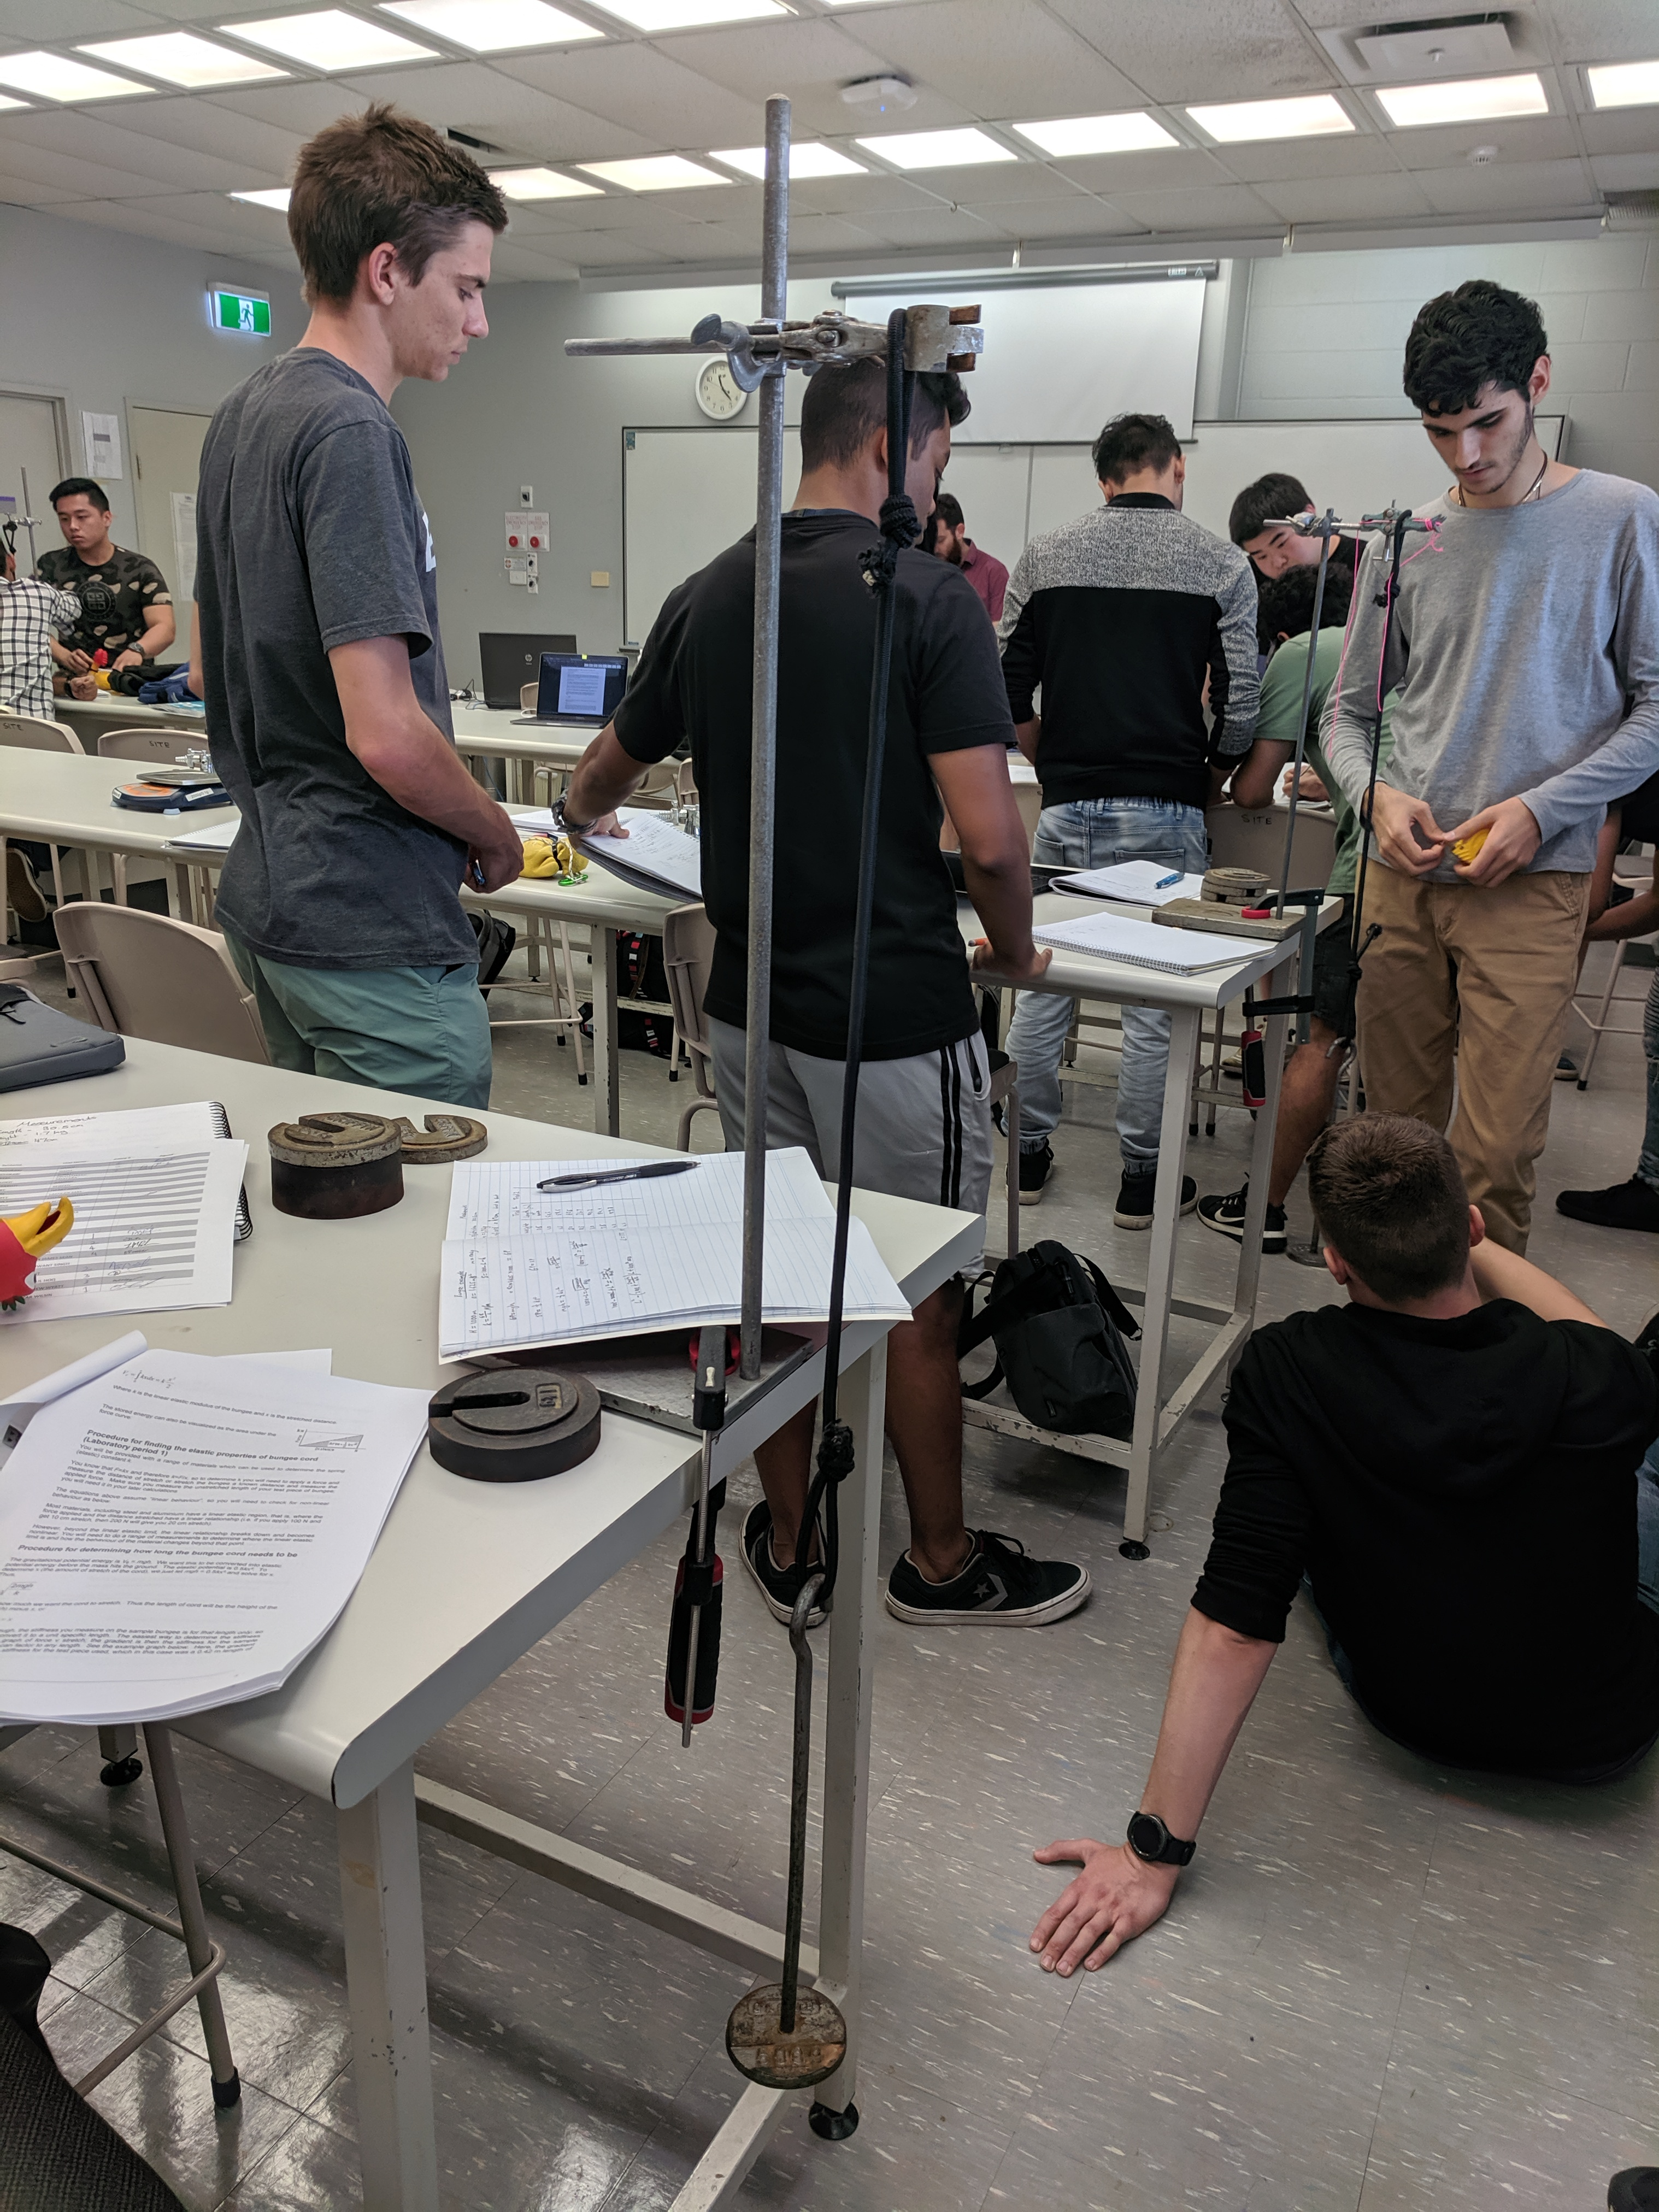
\includegraphics[scale=0.05]{result_1}}
		\caption{A terrible photo of the experimental set up highlighting cramped laboratory conditions often experienced with mass education}
	\end{minipage}
	\hspace{1cm}
	\begin{minipage}{0.45\textwidth}
			\centering
			\captionof{table}{Experimental data on elastic cord material properties were captured by placing successively larger masses on a known length of the cord and measuring the length of the cord at steady state elastic deformation}
			\begin{tabular}{rrr}
				\toprule
				Mass & Length 1 & Length 2\\
				$m$ $[\si{\kilogram}]$ & $\tilde{x}_1$ $[\si{\meter}]$ & $\tilde{x}_2$ $[\si{\meter}]$ \\
				\midrule
				0.00 & 0.47 & 0.47\\
				0.50 & 0.47 & 0.49\\
				1.00 & 0.51 & 0.53\\
				1.50 & 0.60 & 0.63\\
				2.00 & 0.69 & 0.72\\
				2.50 & 0.76 & 0.79\\
				3.00 & 0.80 & 0.83\\
				3.50 & 0.84 & 0.86\\
				4.00 & 0.87 & 0.88\\
				\bottomrule
			\end{tabular}
	\end{minipage}
\end{figure}


\section{Calculations}
Calculations in this practical are comprised of two main parts: determining the stiffness coefficient of the elastic cord used for the bungee jumping chicken; and the calculation of the length of elastic cord to be specified so that the bungee jumping chicken traverses the full balcony height without colliding with the ground.

\subsection{Determining Stiffness Coefficient, $k$}
The spring equation is determined using Hooke's law which states that under elastic deformation a force exerted by a spring, $F_s$, is opposite in direction and proportional to the springs displacement from it's unstretched state, $x$. The proportionality constant, referred to as the stiffness coefficient of the spring, is denoted by $k$. Mathematically the spring equation is expressed in equation (6).
\begin{equation}
F_s = -kx
\end{equation} 

A scatter plot of $(x, F_s)$ pairs can be used to approximate $k$ by fitting a linear model to the data using least squares. Equation (6) highlights that the linear regression model will need to be forced through the origin. To determine $F_s$ we first note that at steady state elastic deformation the mass attached to the elastic cord is at rest. A free body diagram can be seen in Figure 3, where two forces are shown acting on the mass. Acting downwards is the force due to gravity, $F_g$; and acting upwards is an opposing force from the elastic cord, $F_s$. Since the mass is in static equilibrium we can calculate the magnitude of $F_s$ as follows:
\begin{align}
+ \uparrow \sum F &= 0 \nonumber \\
F_s - F_g &= 0 \nonumber \\
\therefore F_s &= F_g
\end{align} 

Since there will be no large excursions from the surface of Earth, it is reasonable to assume that force due to gravity is constant, and gravitational acceleration is equal to $9.81\si{\meter\per\second}$, which we denote by $g$. Given the mass on the cord is known, $F_s$ can be calculated using equation (7) and $F_g = mg$. The force calculations can be seen in Table 2. To determine the 

A short section of elastic cord, approximately $0.47\si{\meter}$ in length, was used to determine the stiffness coefficient, $k$, for this material.
Explain how to conduct the tests for the stiffness check and state the assumptions made constant gravitational acceleration and plastic defomation in materials only.

\begin{figure}[h]
	\begin{minipage}{0.45\textwidth}
		\centering
		\begin{tikzpicture}
			\draw (0,0) circle (1cm);
			\draw[->] (0,0) -- (0,-2);
			\draw[->] (0,1) -- (0,3);
		\end{tikzpicture}
		\caption{text}
	\end{minipage}
	\begin{minipage}{0.45\textwidth}
		\centering
		\captionof{table}{text}
		\begin{tabular}{rrrrr}
			\toprule
			Mass & Force & Disp.  1 & Disp.  2 & Avg. Disp. \\
			$m$ $[\si{\kilogram}]$ & $F$ $[\si{\newton}]$ & $x_1$ $[\si{\meter}]$ & $x_2$ $[\si{\meter}]$ & $x$ $[\si{\meter}]$ \\
			\midrule
			0.00 &  0.00 & 0.00 & 0.00 & 0.00\\
			0.50 &  4.91 & 0.00 & 0.02 & 0.01\\
			1.00 &  9.81 & 0.04 & 0.06 & 0.05\\
			1.50 & 14.72 & 0.13 & 0.16 & 0.14\\
			2.00 & 19.62 & 0.22 & 0.25 & 0.23\\
			2.50 & 24.52 & 0.29 & 0.32 & 0.30\\
			3.00 & 29.43 & 0.33 & 0.36 & 0.35\\
			3.50 & 34.34 & 0.37 & 0.39 & 0.38\\
			4.00 & 39.24 & 0.40 & 0.41 & 0.41\\
			\bottomrule
		\end{tabular}
	\end{minipage}
\end{figure}


State the results seen in section blah were plotted in and linear regression forced through the origin used to fit hooke's law. state the equation
\begin{equation}
F = 90.12x \ \si{\newton}
\end{equation}

\begin{figure}[h]
	\centering
	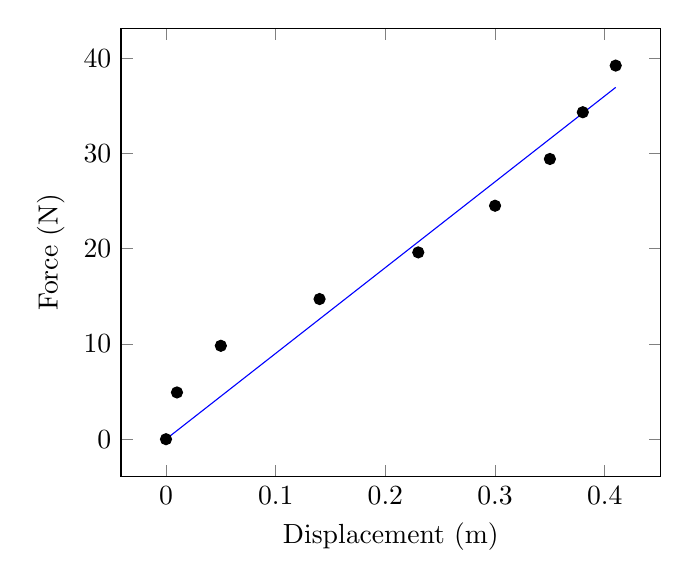
\begin{tikzpicture}
	\begin{axis}[xlabel=Displacement $(\si{\meter})$,
				 ylabel=Force $(\si{\newton})$]
	
	\addplot[only marks] coordinates {
		(0.00, 0.00)
		(0.01, 4.91)
		(0.05, 9.81)
		(0.14, 14.72)
		(0.23, 19.62)
		(0.30, 24.52)
		(0.35, 29.43)
		(0.38, 34.34)
		(0.41, 39.24)
	};
	
	\addplot[no marks, blue, domain=0:0.41] {90.12*x};
	
	\end{axis}
	\end{tikzpicture}
	\caption{text}
\end{figure}

We note a stiffness coefficient of $90.12\si{\newton\per\meter}$ for the $0.47\si{\meter}$ length of bungee cord tested in the lab - this was determined from equation (6). The elastic cord material used for the bungee jumping chicken will be identical to that tested in the lab, however, the specified length will not be $0.47\si{\meter}$ 

\subsection{Predicted Bungee Cord Length}

NEED TO EXPLAIN THE REQUIREMENT OF THE PRACTICAL AND THE SET UP TALK ABOUT THE CHICKEN TOO

Let $h$ be the total height from the balcony rig to the ground; let $x$ be the length of plastic deformation that the cord will undergo for some gravitational potential energy; and let $L$ be the length of unstretched cord. NEED TO MAKE A NOTE ABOUT THE SMALL DISTANCES AND THE LENGTH OF THE CHICKEN and the mass of the chicken too.

We have choice over $L$ and we want to determine this length such that the total unstretched length plus the elastic deformation from the initial potential energy is equal to the height of the balcony. Mathematically this is described by equation (XXXX).
\begin{equation}
h = L + x + l_1 + l_2 + l_3
\end{equation}

This can be written more compactly as:
\begin{equation}
h = \bigg(L + \sum_{i=1}^{3} l_i \bigg) + x
\end{equation}

Graphically this looks like:
\begin{figure}[h]
	\centering
	\begin{minipage}[t]{0.45\textwidth}
		\centering
		\frame{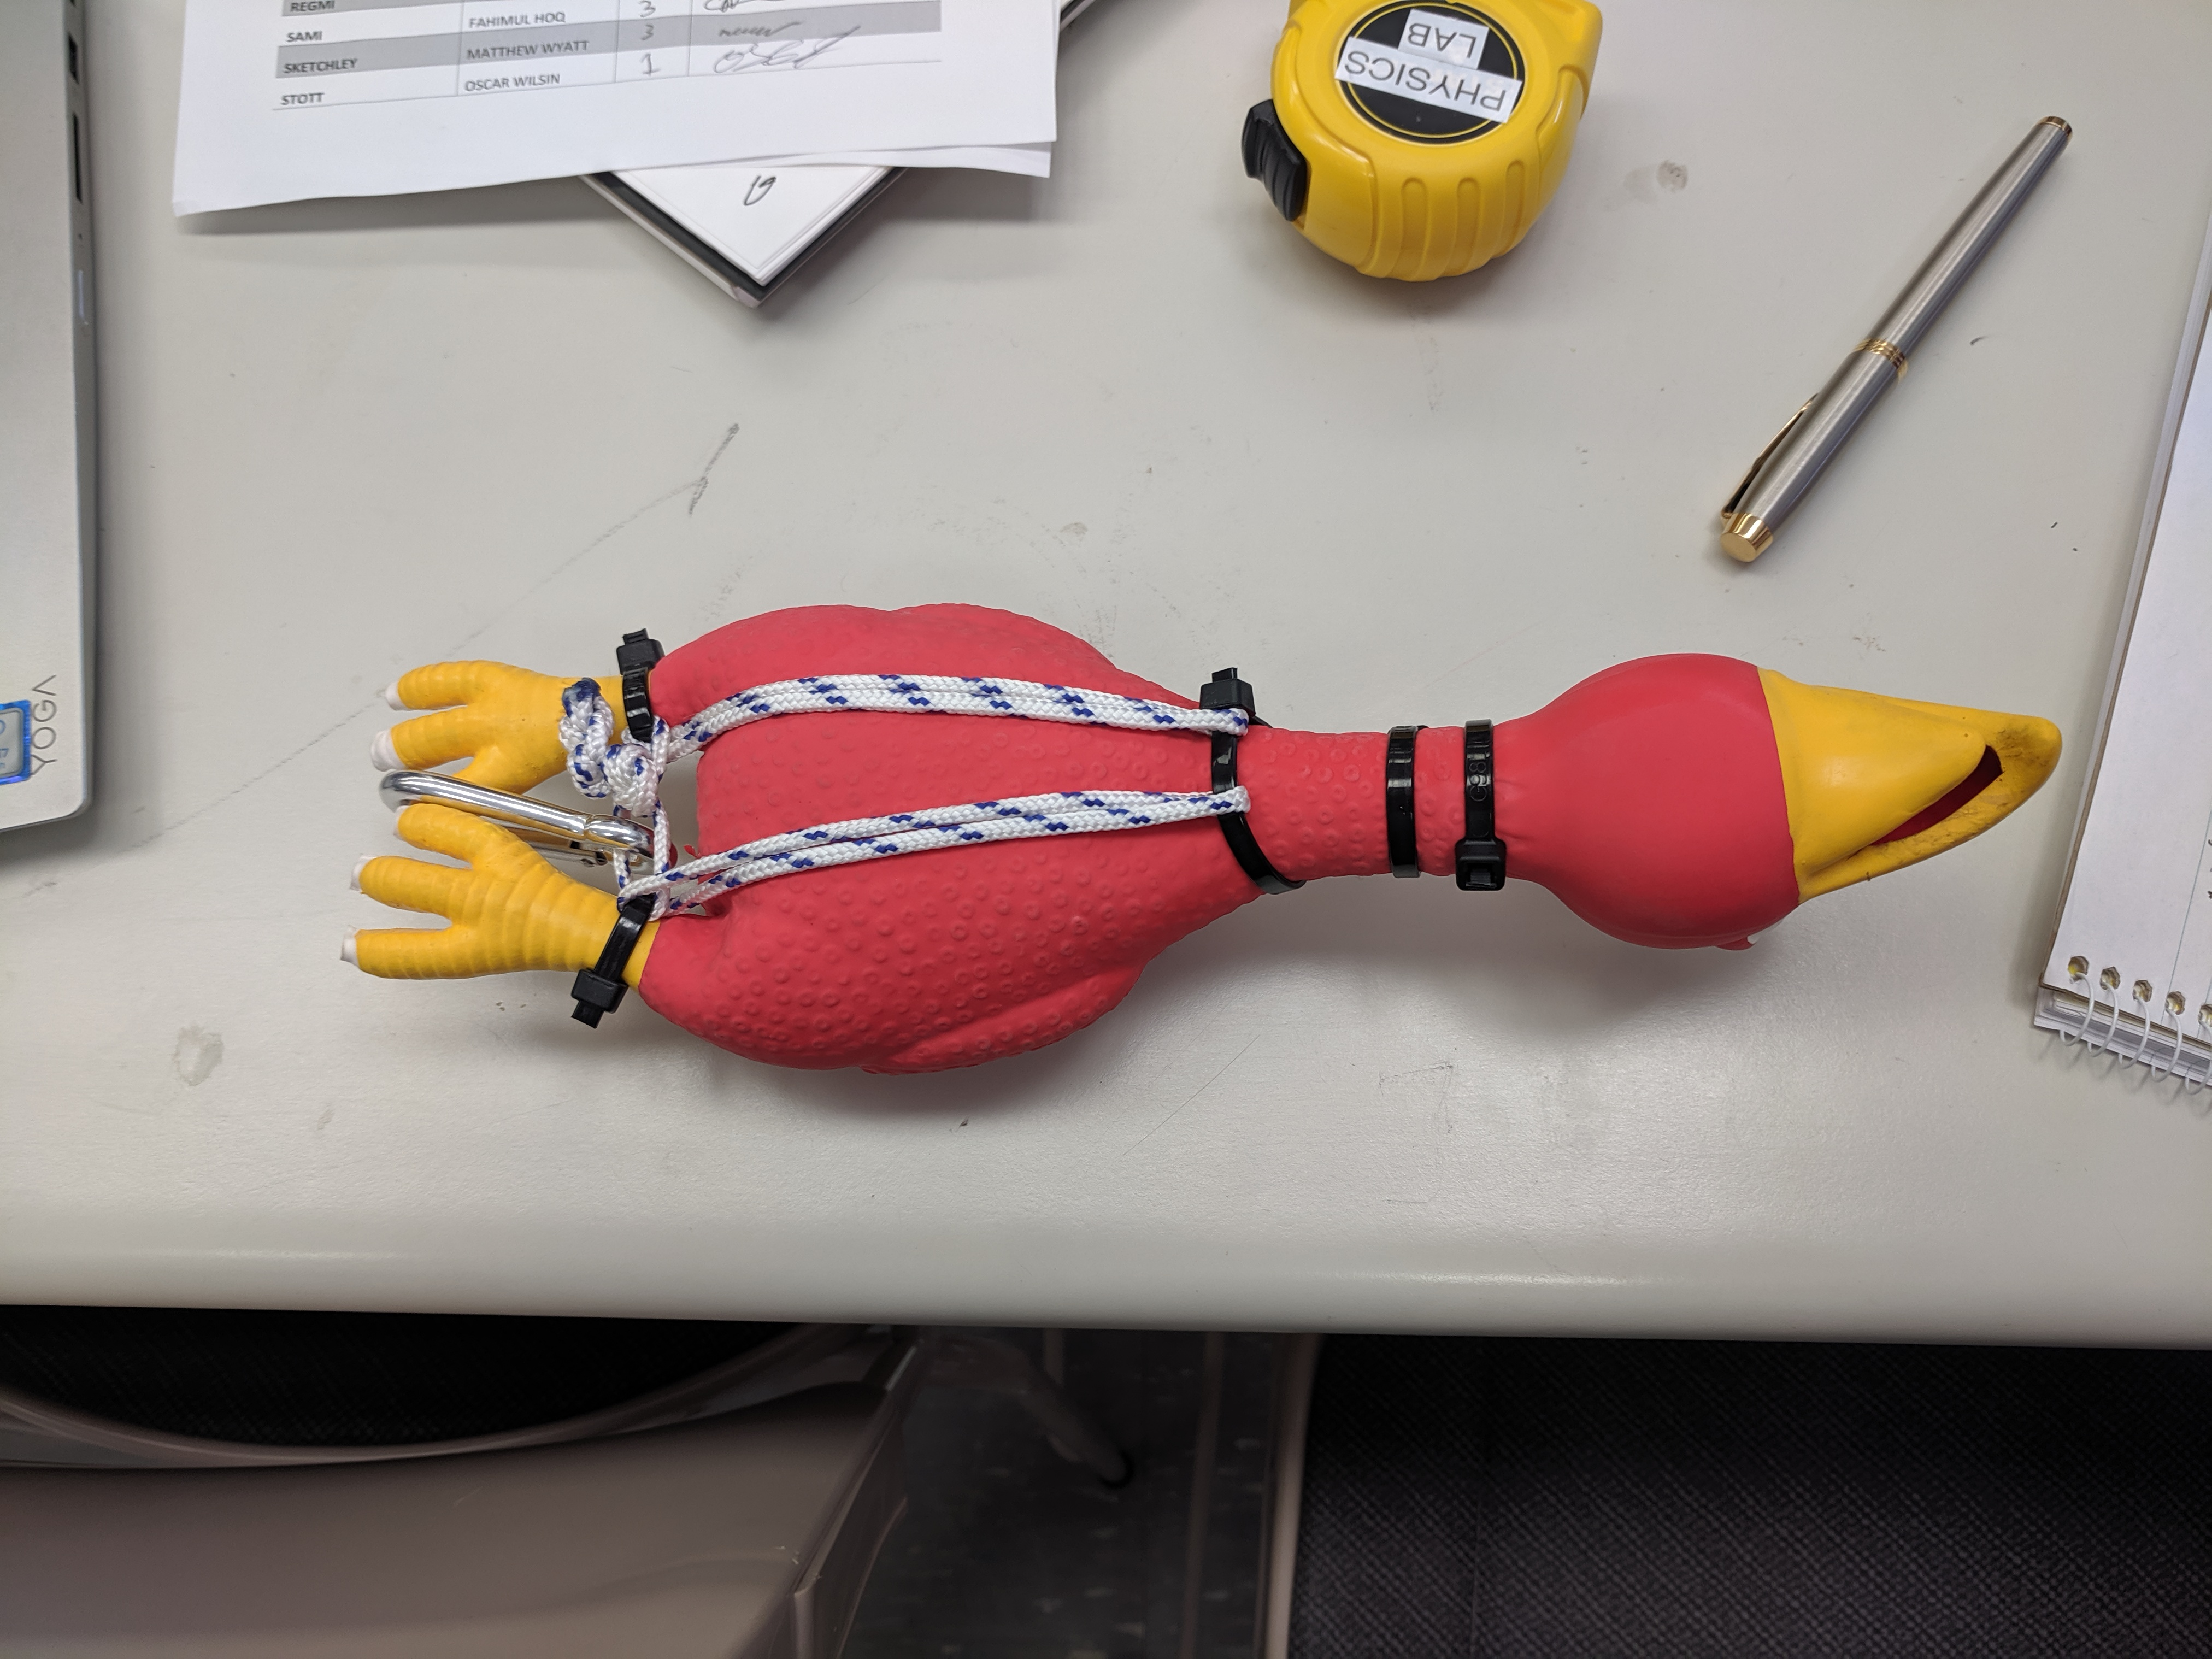
\includegraphics[scale=0.05]{chicken_1}}
		\caption{text}
	\end{minipage}
	\begin{minipage}[t]{0.45\textwidth}
		\centering
		\begin{tikzpicture}
			\draw (0,0) -- (0,-4);
		\end{tikzpicture}
		\caption{text}
	\end{minipage}
\end{figure}

NEED TO PUT A DATUM IN THE DIAGRAM

OR WE COULD TALK SIMPLY ABOUT THE CONDITIONS AT POINT 1 AND POINT 2



As the chicken falls it converts gravitation potential energy into kinetic energy for the full length of the unstretched cord, $L$. At this point the remaining gravitational potential energy and the exiting kinetic energy start to be transferred to elastic potential energy as the elastic cord stretches. As the chicken reaches the full distance $h$, we aim for the chicken to become momentarily stationary. At this point we are assuming that all of the gravitational potential energy, and kinetic energy is transferred to elastic cord
\begin{equation}
(V_g)_1 + (V_e)_1 + T_1 = (V_g)_2 + (V_e)_2 + T_2
\end{equation}

We note that there is no elastic potential at point 1 and the chicken is originally at rest. Similarly, we note that at point 2 there is no gravitational potential energy, and the chicken is again at rest, momentarily. We conclude that $(V_e)_1 = 0 \si{\joule}$, $T_1 = 0 \si{\joule}$, $(V_g)_2 = 0\si{\joule}$, and $T_2 = 0 \si{\joule}$. Equation (XXXX) reduces to

\section{Discussion}

\section{Conclusion}

\bibliography{my_bib}
\bibliographystyle{ieeetr}

\end{document}